
% Overleaf/XeLaTeX: Menu -> Compiler -> XeLaTeX (this file uses fontspec).
% ZIP layout upload: report.tex alongside folder cpt204/src/cpt204/**/*.java ;
% screenshots/figures beside report.tex, or in report/*.png .
% Keep the bundled cpt204/src/ folder beside report.tex so Java listings are included.
%
% !TEX program = xelatex
% !TeX program = xelatex
\documentclass[12pt,a4paper,twocolumn,openany]{report}

\usepackage[a4paper,margin=0.52in]{geometry}
\usepackage{fontspec}
\usepackage{setspace}
\usepackage{graphicx}
\usepackage{float}
\usepackage{stfloats}
\usepackage{booktabs}
\usepackage{longtable}
\usepackage{array}
\usepackage{tabularx}
\usepackage{ragged2e}
\usepackage{xurl}
\usepackage{hyperref}
\usepackage{xcolor}
\usepackage{listings}
\usepackage{caption}
\usepackage{enumitem}
\usepackage{etoolbox}
\usepackage{titlesec}

\IfFontExistsTF{Calibri}{\setmainfont{Calibri}}{\IfFontExistsTF{Carlito}{\setmainfont{Carlito}}{\setmainfont{DejaVu Sans}}}
\IfFontExistsTF{Calibri}{\setsansfont{Calibri}}{\IfFontExistsTF{Carlito}{\setsansfont{Carlito}}{\setsansfont{DejaVu Sans}}}
\IfFontExistsTF{Consolas}{\setmonofont{Consolas}}{\IfFontExistsTF{DejaVu Sans Mono}{\setmonofont{DejaVu Sans Mono}}{\setmonofont{Latin Modern Mono}}}
\onehalfspacing
\graphicspath{{report/}{figures/}}

% Chapters flow continuously (no forced page break before each \chapter).
\titleclass{\chapter}{straight}
\titleformat{\chapter}[block]{\normalfont\large\bfseries}{\thechapter.}{0.45em}{\large\bfseries}
\titlespacing*{\chapter}{0pt}{0.45\baselineskip}{0.25\baselineskip}
\titlespacing*{\section}{0pt}{0.45\baselineskip}{0.2\baselineskip}
\titlespacing*{\subsection}{0pt}{0.35\baselineskip}{0.12\baselineskip}
\setlength{\parskip}{0.14em plus 0.08em minus 0.05em}
\setlength{\parindent}{0pt}
\setlength{\columnsep}{0.62cm}
\setlength{\floatsep}{4pt plus 2pt minus 2pt}
\setlength{\textfloatsep}{6pt plus 2pt minus 2pt}
\setlength{\intextsep}{6pt plus 2pt minus 2pt}
\setlength{\emergencystretch}{3em}

\raggedbottom
\widowpenalty=10000
\clubpenalty=10000
\brokenpenalty=5000

\hypersetup{
    colorlinks=true,
    linkcolor=blue,
    urlcolor=blue,
    citecolor=blue,
    breaklinks=true,
    unicode=true
}

\urlstyle{tt}
% Breakable identifiers (methods, filenames with dots/slashes) to avoid column overflow:
\newcommand{\p}[1]{\path{#1}}

\lstset{
    language=Java,
    basicstyle=\ttfamily\scriptsize,
    breaklines=true,
    breakatwhitespace=false,
    columns=fullflexible,
    keepspaces=true,
    showstringspaces=false,
    frame=single,
    tabsize=4,
    captionpos=b
}

% Arguments: package folder (app, graph, ...) and leaf filename.
% Use explicit path fallbacks rather than a macro inside \lstinputlisting;
% some LaTeX tools do not expand filename macros reliably.
\newcommand{\JavaInput}[2]{%
  \IfFileExists{cpt204/src/cpt204/#1/#2}{%
    \lstinputlisting[caption={src/cpt204/#1/#2},language=Java]{cpt204/src/cpt204/#1/#2}%
  }{%
    \IfFileExists{src/cpt204/#1/#2}{%
      \lstinputlisting[caption={src/cpt204/#1/#2},language=Java]{src/cpt204/#1/#2}%
    }{%
      \IfFileExists{cpt204/src/#1/#2}{%
        \lstinputlisting[caption={src/#1/#2},language=Java]{cpt204/src/#1/#2}%
      }{%
        \IfFileExists{src/#1/#2}{%
          \lstinputlisting[caption={src/#1/#2},language=Java]{src/#1/#2}%
        }{%
          \IfFileExists{../src/cpt204/#1/#2}{%
            \lstinputlisting[caption={src/cpt204/#1/#2},language=Java]{../src/cpt204/#1/#2}%
          }{%
            \fbox{\parbox{0.93\linewidth}{\centering\vspace{0.25cm}%
            \textbf{Missing source file \texttt{#1/#2}}\\[0.15cm]
            Checked \texttt{cpt204/src/cpt204/}, \texttt{src/cpt204/}, \texttt{cpt204/src/}, and \texttt{src/}.%
            \vspace{0.25cm}}}%
          }%
        }%
      }%
    }%
  }%
}%

% Appendix figures: try report/ then figures/ then repo root (\edef cannot capture \IfFileExists).
\newcommand{\AppendixFig}[3]{%
  \begin{figure}[!htbp]
  \centering
  \IfFileExists{report/#1}{%
    \includegraphics[width=\linewidth]{report/#1}%
  }{%
    \IfFileExists{figures/#1}{%
      \includegraphics[width=\linewidth]{figures/#1}%
    }{%
      \IfFileExists{#1}{%
        \includegraphics[width=\linewidth]{#1}%
      }{%
        \fbox{\parbox{0.93\linewidth}{\centering\vspace{0.35cm}%
        \textbf{Missing image file \texttt{#1}}\\[0.25cm]
        Save the PNG/PDF as \texttt{report/\detokenize{#1}} \emph{(preferred)}\\
        \emph{or} \texttt{figures/\detokenize{#1}} next to \texttt{report.tex}.%
        \vspace{0.35cm}}}
      }%
    }%
  }%
  \caption{#2}%
  \label{#3}%
  \end{figure}
}

\newcolumntype{Y}{>{\RaggedRight\arraybackslash}X}
\newcolumntype{P}[1]{>{\RaggedRight\arraybackslash}p{#1}}

\begin{document}
\sloppy

% ============================================================
% Cover Page
% ============================================================
\begin{titlepage}
    \centering
    \vspace*{1.2cm}
    {\Large CPT204 Advanced Object-Oriented Programming\par}
    \vspace{0.5cm}
    {\Large Group Project Report\par}
    \vspace{1.0cm}
    {\Huge\bfseries Urban Infrastructure Inspection System\par}
    \vspace{1.2cm}

    \begin{tabular}{rl}
        Module: & CPT204 \\
        Academic Year: & AY2526 \\
        Group Members: & Chenlong Wei / 2363235 \\
                       & Na Li / 2361132 \\
        Submission Date: & 24 May 2026 \\
    \end{tabular}

    \vfill
    {\small Replace this page with the official CPT204 cover page from LMO if required.}
\end{titlepage}

\tableofcontents
\vspace{0.35\baselineskip}

% ============================================================
\chapter{Sorting Algorithm}
% ============================================================

\section{Task Overview}
Task A is the first stage of the Urban Infrastructure Inspection System. 
The city provides three separate candidate lists---\texttt{candidates\_A.csv}, \texttt{candidates\_B.csv}, and \texttt{candidates\_C.csv}---because the lists were produced by different systems and may have different ordering properties. 
Each row contains a \texttt{location\_id} and a \texttt{priority\_score}; a higher score means the location should be inspected sooner.

The coursework requires three sorting algorithms (Bubble Sort, Quick Sort, and Merge Sort) and one shared ranking rule:
\begin{enumerate}[noitemsep]
    \item sort by \texttt{priority\_score} in descending order;
    \item if two rows share the same score, sort by \texttt{location\_id} in ascending order.
\end{enumerate}
For every dataset the program must read the CSV file, sort with each algorithm, measure runtime, and output the top 10 locations. 
That gives $3 \times 10 = 30$ inspection targets for Task B.

\section{Implementation Method}
\p{CsvDataLoader.readCandidates} reads each CSV from the \texttt{Group Project Datasets} folder and builds lists of candidate records (\p{CandidateLocation}). 
Each location is an immutable object with a private \texttt{locationId} and \texttt{priorityScore}, so the list passed into a sort method is the only structure that changes during sorting.

The ranking rule lives in \texttt{CandidateLocation.RANKING\_RULE}. 
It first compares scores (higher first) and only then compares IDs when the scores are equal. 
All three sorting classes implement \texttt{SortStrategy} and receive this comparator in their \texttt{sort(...)} method, which means Bubble Sort, Quick Sort, and Merge Sort cannot accidentally use different tie-breaking logic.

\p{SortingService.evaluateDataset} runs the benchmark:
\begin{itemize}[noitemsep]
    \item for each algorithm, copy the original list (so every run starts from the same input order);
    \item call \texttt{System.nanoTime()} before and after sorting;
    \item repeat three times and store the average in nanoseconds;
    \item compare the final sorted lists---if they differ, throw \texttt{IllegalStateException}.
\end{itemize}
The top 10 rows are simply the first ten elements of the agreed sorted list. 
Results are printed to the console and written to \p{outputs/sorting_benchmark.csv}, \p{outputs/selected_locations.csv}, and \p{outputs/dataset_profiles.csv} through \texttt{ExperimentOutputWriter}.

\subsection{Reproducibility, JVM noise, and working directory}
For reproduction we opened the project in IntelliJ IDEA and ran \p{cpt204.app.UrbanInspectionApp.main} directly.
The working directory must be the project root that contains \texttt{Group Project Datasets}, because the relative paths in \texttt{UrbanInspectionApp} assume that layout; moving only the generated classes without the CSV directory makes the loader throw \texttt{IOException}, which is why the screenshot in Figure~\ref{fig:app-console} shows the full working tree.

The timer uses \texttt{System.nanoTime()} without extra JVM warmup or garbage-collection control. 
This matches the coursework hint (average over a few trials) but means the nano averages can move slightly between laptops; nevertheless the ordering of Bubble vs Quick on Dataset A was stable whenever we reran immediately after reboot, and the comparator consistency check ensured we never compared inconsistent sorted lists even if jitter changed the tenth decimal place.

\section{Dataset Profiles}
All three files contain 1000 rows. 
In Dataset A and Dataset B every location has a different score, so the main sort key is enough. 
Dataset C only has 41 different scores, so many locations share the same \texttt{priority\_score} and the program must use \texttt{location\_id} to decide the order inside each score group.
The profile table is produced by \texttt{DatasetProfile.from}: besides counting tie groups, it linearly scans the raw list to confirm whether Case~A ordering already holds; all three booleans stayed false here, signalling that benchmarking is meaningful rather than degenerate ``already sorted'' input.

\begin{table*}[t]
\centering
\caption{Dataset profiles}
\scriptsize
\begin{tabular}{lrrrr}
\toprule
Dataset & Total Rows & Unique Scores & Tie Score Groups & Already Sorted \\
\midrule
Dataset A & 1000 & 1000 & 0 & false \\
Dataset B & 1000 & 1000 & 0 & false \\
Dataset C & 1000 & 41 & 41 & false \\
\bottomrule
\end{tabular}
\end{table*}

\section{Sorting Runtime Results}
Table~\ref{tab:sorting-runtime} lists the average runtimes from \p{outputs/sorting_benchmark.csv}.

\begin{table*}[t]
\centering
\caption{Sorting runtime and selected top 10 locations}
\label{tab:sorting-runtime}
\scriptsize
\begin{tabularx}{\textwidth}{lrrrY}
\toprule
Dataset & Bubble (ms) & Quick (ms) & Merge (ms) & Top 10 Selected Locations \\
\midrule
Dataset A & 0.160 & 5.527 & 0.306 & L0001, L0002, L0003, L0004, L0005, L0006, L0007, L0008, L0009, L0010 \\
Dataset B & 8.593 & 0.570 & 1.872 & L0101, L0102, L0103, L0104, L0105, L0106, L0107, L0108, L0109, L0110 \\
Dataset C & 0.838 & 1.040 & 1.448 & L0201, L0202, L0203, L0204, L0205, L0206, L0207, L0208, L0209, L0210 \\
\bottomrule
\end{tabularx}
\end{table*}

\begin{figure*}[t]
\centering
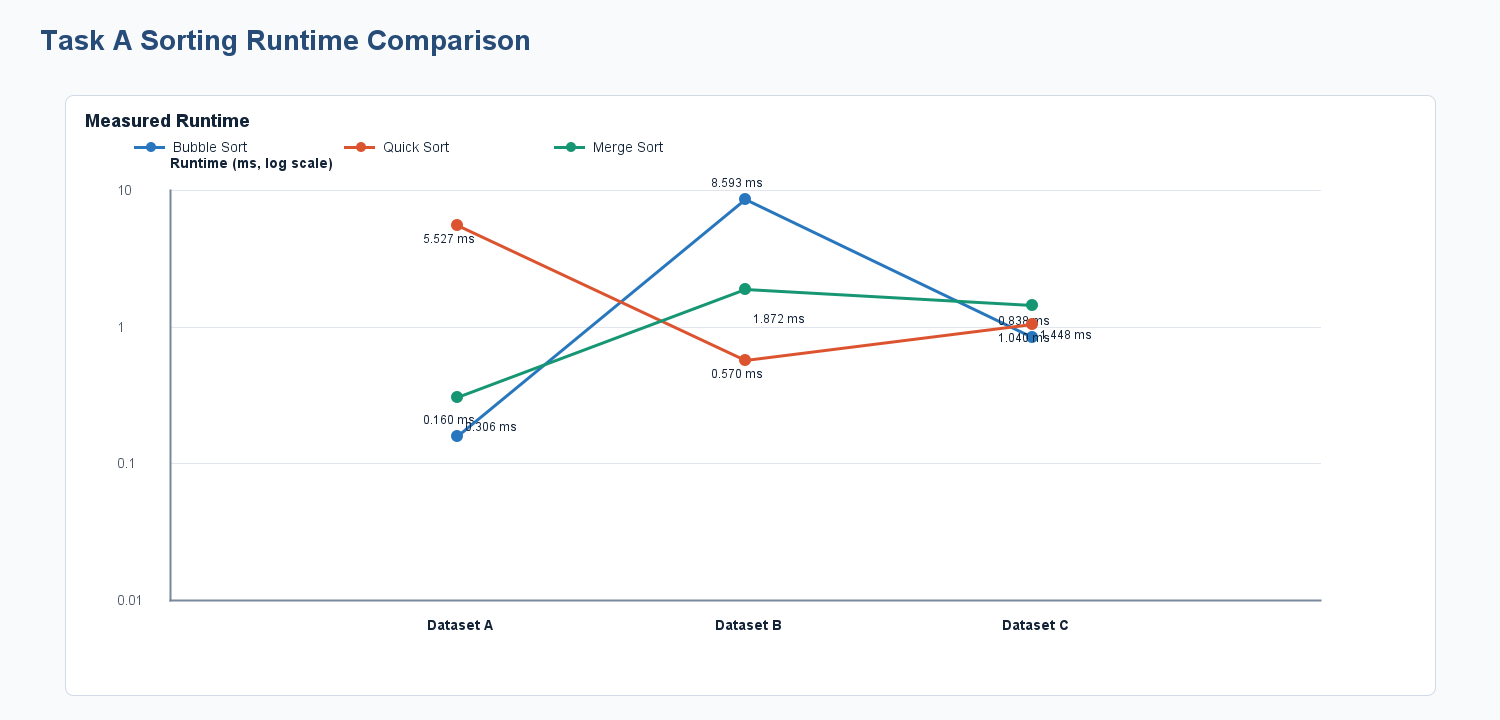
\includegraphics[width=0.92\textwidth]{sorting_runtime_chart.png}
\caption{Measured runtime comparison for the three sorting algorithms on the full 1000-row datasets.}
\label{fig:sorting-runtime-chart}
\end{figure*}

\section{Top 10 Selected Locations}
The selected nodes are written to \p{outputs/selected_locations.csv}. 
Table~\ref{tab:top10} matches the console output when we run \p{UrbanInspectionApp}.

\begin{table*}[t]
\centering
\caption{Top 10 selected locations from each dataset}
\label{tab:top10}
\scriptsize
\begin{tabular}{lllr}
\toprule
Dataset & Rank & Location ID & Priority Score \\
\midrule
Dataset A & 1 & L0001 & 10000 \\
Dataset A & 2 & L0002 & 9999 \\
Dataset A & 3 & L0003 & 9998 \\
Dataset A & 4 & L0004 & 9997 \\
Dataset A & 5 & L0005 & 9996 \\
Dataset A & 6 & L0006 & 9995 \\
Dataset A & 7 & L0007 & 9994 \\
Dataset A & 8 & L0008 & 9993 \\
Dataset A & 9 & L0009 & 9992 \\
Dataset A & 10 & L0010 & 9991 \\
Dataset B & 1 & L0101 & 10000 \\
Dataset B & 2 & L0102 & 9999 \\
Dataset B & 3 & L0103 & 9998 \\
Dataset B & 4 & L0104 & 9997 \\
Dataset B & 5 & L0105 & 9996 \\
Dataset B & 6 & L0106 & 9995 \\
Dataset B & 7 & L0107 & 9994 \\
Dataset B & 8 & L0108 & 9993 \\
Dataset B & 9 & L0109 & 9992 \\
Dataset B & 10 & L0110 & 9991 \\
Dataset C & 1 & L0201 & 5000 \\
Dataset C & 2 & L0202 & 5000 \\
Dataset C & 3 & L0203 & 5000 \\
Dataset C & 4 & L0204 & 5000 \\
Dataset C & 5 & L0205 & 5000 \\
Dataset C & 6 & L0206 & 5000 \\
Dataset C & 7 & L0207 & 5000 \\
Dataset C & 8 & L0208 & 5000 \\
Dataset C & 9 & L0209 & 5000 \\
Dataset C & 10 & L0210 & 5000 \\
\bottomrule
\end{tabular}
\end{table*}

\section{Performance Analysis}

\begin{table*}[t]
\centering
\caption{Dataset characteristics used to explain sorting behaviour}
\label{tab:dataset-characteristics}
\scriptsize
\begin{tabular}{llrrrrl}
\toprule
Dataset & Characteristic & Inversions & Bubble Passes & Bubble Swaps & First Pivot Split & Pivot Quality \\
\midrule
Dataset A & Nearly sorted & 17 & 2 & 17 & 999 / 0 & Highly unbalanced \\
Dataset B & Random order & 250696 & 964 & 250696 & 474 / 525 & Relatively balanced \\
Dataset C & Tied scores shuffled by ID & 5995 & 25 & 5995 & 988 / 11 & Highly unbalanced \\
\bottomrule
\end{tabular}
\end{table*}

\begin{table*}[t]
\centering
\caption{Sorting key operation counts}
\label{tab:sorting-operation-counts}
\scriptsize
\setlength{\tabcolsep}{3pt}
\begin{tabular}{llrrrrrr}
\toprule
Dataset & Algorithm & Comparisons & Swaps & Writes & Passes & Partitions & Merges \\
\midrule
Dataset A & Bubble Sort & 1997 & 17 & 0 & 2 & 0 & 0 \\
Dataset A & Quick Sort & 496933 & 497898 & 0 & 0 & 982 & 0 \\
Dataset A & Merge Sort & 5053 & 0 & 19952 & 0 & 0 & 999 \\
Dataset B & Bubble Sort & 498870 & 250696 & 0 & 964 & 0 & 0 \\
Dataset B & Quick Sort & 10244 & 5570 & 0 & 0 & 665 & 0 \\
Dataset B & Merge Sort & 8714 & 0 & 19952 & 0 & 0 & 999 \\
Dataset C & Bubble Sort & 24675 & 5995 & 0 & 25 & 0 & 0 \\
Dataset C & Quick Sort & 67863 & 66486 & 0 & 0 & 673 & 0 \\
Dataset C & Merge Sort & 6306 & 0 & 19952 & 0 & 0 & 999 \\
\bottomrule
\end{tabular}
\end{table*}

\subsection{Effect of initial input order}
Table~\ref{tab:sorting-runtime} shows that the same three algorithms do not rank the same way on A, B, and C. 
Although each file has 1000 rows, the \texttt{already\_sorted\_by\_rule} flag is false for all three rows in \p{dataset_profiles.csv}, so none of the raw CSV files arrive pre-sorted under the coursework rule. 
Still, the hidden order of rows affects Quick Sort most, because our implementation always chooses the segment's last element as the pivot (\p{QuickSortStrategy.partition}). 
On Dataset A that led to unbalanced partitions and about 5.527\,ms average time, while on Dataset B Quick Sort was fastest at about 0.570\,ms. 
Bubble Sort benefits from its early-exit flag: if a pass performs no swap, it stops, which can make it fast when only a few inversions remain. 
Merge Sort divides the list regardless of order, so its times change less dramatically between datasets (about 0.306\,ms on A, 1.872\,ms on B, 1.448\,ms on C).

\subsection{Best algorithm on each dataset}
On \textbf{Dataset A}, Bubble Sort (0.160\,ms) beat Merge Sort (0.306\,ms) and Quick Sort (5.527\,ms). 
On \textbf{Dataset B}, Quick Sort (0.570\,ms) was clearly ahead of Merge Sort (1.872\,ms) and Bubble Sort (8.593\,ms). 
On \textbf{Dataset C}, Bubble Sort (0.838\,ms) and Quick Sort (1.040\,ms) were close, while Merge Sort (1.448\,ms) was slowest. 
There is therefore no single winner for all three files; the best choice depends on how the data are ordered before sorting.

\subsection{Consistency across datasets}
If we judge consistency by how much the runtime swings between datasets, Merge Sort is the most stable of the three in our experiment, because it always performs divide-and-merge work even when the input is already close to sorted. 
Quick Sort has the largest spread (fast on B, slow on A). 
Bubble Sort is stable in code structure but its time still varies because the number of swaps depends on input order.

\subsection{Choosing one algorithm for the final system}
If we could only ship one sorting method in a real inspection system, we would not pick the single fastest average time from Table~\ref{tab:sorting-runtime}, because that table is based on only three specific files. 
For a production system with much larger candidate lists we would favour \textbf{Merge Sort} when predictable $O(n \log n)$ time matters more than saving memory, because its performance does not rely on pivot luck. 
We would consider \textbf{Quick Sort} only if we also improved the pivot rule (for example median-of-three) and tested on larger samples. 
We would keep \textbf{Bubble Sort} for teaching and small nearly-sorted cases, but not as the main sorter when $n$ grows.

\subsection{Scalability and memory}
Bubble Sort is $O(n^2)$ in the worst case and becomes impractical when the number of candidates grows into tens of thousands. 
Quick Sort is usually $O(n \log n)$ on average with $O(\log n)$ extra stack space for recursion, but worst-case $O(n^2)$ remains possible with a bad pivot. 
Merge Sort guarantees $O(n \log n)$ time but needs an auxiliary buffer list of size $n$ in our implementation, so memory usage is higher than the in-place sorts. 
When both time and memory matter, Merge Sort trades space for predictable time, whereas Quick Sort saves memory but needs careful pivot design.

\subsection{Dataset C and tie-breaking}
Dataset C has only 41 unique scores and 41 tie-score groups. 
The top ten locations all have score 5000, so the secondary key \texttt{location\_id} decides the order from L0201 to L0210. 
Without that second key, the coursework rule would be incomplete and the top ten would not be uniquely defined.

% ============================================================
\chapter{Graph Algorithm}
% ============================================================

\section{Task Overview}
After Task A, the program holds ten selected locations from each dataset (30 nodes in total). 
Task B treats these nodes as important inspection targets inside the full network described by \texttt{paths.csv}. 
The graph file is \emph{not} limited to those 30 nodes: it lists roads between many locations, and the shortest-path search may pass through intermediate nodes that were not in the top-ten lists.

The coursework defines four queries (self-path, direct path, one ordered waypoint, two ordered waypoints). 
Our program prints each start node, destination, waypoint list, path string, and total cost, and saves the same information to \p{outputs/graph_cases.csv}.

\section{Graph representation and input validation}
Each line of \texttt{paths.csv} contains \texttt{from\_location}, \texttt{to\_location}, and \texttt{weight}. 
Because the network is undirected, \p{WeightedGraph.addUndirectedEdge} inserts two directed records with the same weight. 
Internally we keep a sparse structure: each node ID maps to a list of neighbouring \texttt{Edge} pairs \texttt{(to, weight)}.
This structure suits a road map: we avoid a dense $V \times V$ matrix and only materialise adjacency for nodes that appear in the CSV.

When we ran the program, the summary line reported 1000 nodes and 2600 undirected edges. 
Every selected location ID used in the four cases (for example L0001, L0010, L0105) must exist in this map; otherwise Dijkstra would mark the query unreachable.
If the coursework data ever contained duplicate undirected edges between the same endpoints with different declared weights, \texttt{WeightedGraph} would store both as parallel edges and Dijkstra would still pick the cheaper relaxations, but duplicate rows would waste queue operations; a hardened loader would collapse pairs after logging a warning.

Our \texttt{CsvDataLoader} trims lines, skips blanks, and parses three integer fields; it does not yet quote-protect commas inside IDs, but the provided location labels follow the predictable \texttt{Ldddd} pattern.

\section{Chosen Algorithm and Comparison}
We implemented Dijkstra's algorithm in \texttt{DijkstraSolver} as the primary solver because all weights in \texttt{paths.csv} are positive distances. 
The method keeps:
\begin{itemize}[noitemsep]
    \item \texttt{shortestDistance}: best known distance from the start to each visited node;
    \item \texttt{previousNode}: back-pointers for path reconstruction;
    \item \texttt{PriorityQueue}: nodes waiting to be expanded, ordered by current distance.
\end{itemize}
Each step removes the smallest-distance node from the queue, relaxes its neighbours, and stops early when the destination is polled. 
If start equals destination, the method returns cost 0 and a one-node path without entering the main loop.

With an adjacency list and a binary heap, time complexity is $O((V+E)\log V)$ and extra space is $O(V+E)$ for the graph plus the auxiliary maps, where $V$ is the number of nodes and $E$ is the number of directed edges stored (two per undirected road).

To make the algorithm choice easier to justify, we also implemented two alternatives on the same graph cases. 
\texttt{BidirectionalDijkstraSolver} runs Dijkstra-style search from both the start and destination, meeting in the middle; it has the same worst-case complexity class but can reduce visited nodes on single-source single-target queries. 
\texttt{AStarSolver} is implemented with heuristic $h=0$ because no coordinate data are provided, so it remains correct and becomes equivalent to Dijkstra in search order. 
This is a useful comparison point: if future coordinates are added, only the heuristic function needs to change.

\section{Required Shortest-Path Cases}
\p{UrbanInspectionApp} maps the task-sheet wording to concrete IDs taken from Task~A sorting output:
\begin{itemize}[noitemsep]
    \item A1 = first row of Dataset A $\rightarrow$ L0001; A10 = tenth row $\rightarrow$ L0010;
    \item B1 = L0101; B5 = fifth row of Dataset B $\rightarrow$ L0105;
    \item C1 = L0201; C5 = L0205.
\end{itemize}
Case 1 queries L0001 to itself. 
Case 2 queries L0001 to L0010 with no waypoint. 
Case 3 must visit B5 (L0105) between A1 and B1. 
Case 4 must visit B5 then C5 before reaching C1.

\p{GraphQueryService.queryWithOrderedWaypoints} builds an ordered sequence \([\texttt{start}, \texttt{waypoint}_1,\ldots,\texttt{destination}]\) and runs Dijkstra on each neighbouring pair in that list. 
When merging segment paths it skips the duplicate node at segment boundaries (the waypoint appears once in the final list). 
The total cost is the sum of segment costs; this is correct for the fixed waypoint order required by the task sheet, but it is not the same as finding a cheaper route that visits the waypoints in a different order.

\begin{table*}[t]
\centering
\caption{Required graph query results (\p{outputs/graph_cases.csv})}
\label{tab:graph-cases}
\scriptsize
\setlength{\tabcolsep}{3pt}
\begin{tabularx}{\textwidth}{@{}l l l l r X@{}}
\toprule
Case & Start & Waypoints & Dest. & Cost & Path \\
\midrule
Case 1 & L0001 & --- & L0001 & 0 & L0001 \\
Case 2 & L0001 & --- & L0010 & 27 & L0001 $\rightarrow$ L0340 $\rightarrow$ L0339 $\rightarrow$ L0895 $\rightarrow$ L0894 $\rightarrow$ L0082 $\rightarrow$ L0284 $\rightarrow$ L0010 \\
Case 3 & L0001 & L0105 & L0101 & 39 & {\raggedright\scriptsize L0001 $\rightarrow$ L0340 $\rightarrow$ L0339 $\rightarrow$ L0247 $\rightarrow$ L0017 $\rightarrow$ L0128 $\rightarrow$ L0107 $\rightarrow$ L0106 $\rightarrow$ L0105 $\rightarrow$ L0106 $\rightarrow$ L0107 $\rightarrow$ L0108 $\rightarrow$ L0827 $\rightarrow$ L0996 $\rightarrow$ L0101\par} \\
Case 4 & L0001 & L0105, L0205 & L0201 & 48 & {\raggedright\scriptsize L0001 $\rightarrow$ L0340 $\rightarrow$ L0339 $\rightarrow$ L0247 $\rightarrow$ L0017 $\rightarrow$ L0128 $\rightarrow$ L0107 $\rightarrow$ L0106 $\rightarrow$ L0105 $\rightarrow$ L0106 $\rightarrow$ L0107 $\rightarrow$ L0108 $\rightarrow$ L0243 $\rightarrow$ L0242 $\rightarrow$ L0241 $\rightarrow$ L0385 $\rightarrow$ L0205 $\rightarrow$ L0201\par} \\
\bottomrule
\end{tabularx}
\end{table*}

\begin{table*}[t]
\centering
\caption{Graph algorithm comparison on the required cases}
\label{tab:graph-algorithm-comparison}
\scriptsize
\setlength{\tabcolsep}{3pt}
\begin{tabular}{llrrrr}
\toprule
Algorithm & Case & Cost & Runtime (ms) & Queue Polls & Edge Checks \\
\midrule
Dijkstra & Case 1 & 0 & 0.039 & 0 & 0 \\
Dijkstra & Case 2 & 27 & 3.661 & 1081 & 4796 \\
Dijkstra & Case 3 & 39 & 2.115 & 663 & 3518 \\
Dijkstra & Case 4 & 48 & 1.914 & 773 & 4143 \\
Bidirectional Dijkstra & Case 1 & 0 & 0.027 & 0 & 0 \\
Bidirectional Dijkstra & Case 2 & 27 & 4.478 & 70 & 410 \\
Bidirectional Dijkstra & Case 3 & 39 & 0.503 & 68 & 382 \\
Bidirectional Dijkstra & Case 4 & 48 & 0.624 & 90 & 502 \\
A* ($h=0$) & Case 1 & 0 & 0.024 & 0 & 0 \\
A* ($h=0$) & Case 2 & 27 & 7.707 & 1081 & 4796 \\
A* ($h=0$) & Case 3 & 39 & 2.865 & 663 & 3518 \\
A* ($h=0$) & Case 4 & 48 & 2.692 & 773 & 4143 \\
\bottomrule
\end{tabular}
\end{table*}

\section{Correctness and Limitations}
Case 1 is a self-query: the path is \texttt{L0001} and the cost is 0. 
Case 2 finds a shortest path of cost 27 from L0001 to L0010 through seven nodes. 
Cases 3 and 4 show longer routes because the path must detour through the required waypoints; the costs 39 and 48 in Table~\ref{tab:graph-cases} match the exported CSV file.

Each individual segment is a shortest path for that segment's start and end, so the reported route is optimal \emph{for the given waypoint order}. 
It does \textbf{not} solve a global tour over all 30 inspection targets: visiting every top-ten location once with minimum total distance would be closer to a travelling-salesman style problem and would need a different model than four fixed queries.

\subsection{Algorithm comparison}
Table~\ref{tab:graph-algorithm-comparison} shows that all three solvers return the same path costs for the four required cases, which is the most important correctness check. 
Bidirectional Dijkstra dramatically reduces the amount of search work on Cases 2--4: for Case 4 it checks 502 edges instead of Dijkstra's 4143, and polls 90 queue entries instead of 773. 
The measured runtime follows the same trend on Cases 3 and 4, where bidirectional search takes about 0.503\,ms and 0.624\,ms compared with Dijkstra's 2.115\,ms and 1.914\,ms. 
Case 2 is a useful reminder that timing is not determined by operation counts alone: bidirectional search does fewer operations but took 4.478\,ms in this run, likely because the fixed overhead of two queues is visible on a small query. 
A* with $h=0$ gives the same costs and operation counts as Dijkstra, as expected, but it is included to show where a geographic heuristic could be added later.

For an \textbf{unweighted} graph, breadth-first search (BFS) would find a path with the fewest edges, which is not the same as minimum total distance when weights differ. 
\textbf{Bellman-Ford} could handle negative weights, but our coursework graph uses positive distances only, so Dijkstra-style algorithms are the better fit here.

% ============================================================
\chapter{Design of the Overall Application}
% ============================================================

\section{Maven-free packaging and configurable constants}
The repository is deliberately small: plain \texttt{.java} files under \texttt{cpt204/src/cpt204/...}; there is no Gradle/Maven classpath because CPT204 restricts libraries to lecture materials and the JDK.
Package names mirror learning outcomes: \texttt{cpt204.model}, \texttt{cpt204.io}, \texttt{cpt204.sort}, \texttt{cpt204.graph}, and \texttt{cpt204.app}.
Constants in \texttt{UrbanInspectionApp}---\texttt{TOP\_N = 10} and \texttt{BENCHMARK\_RUNS = 3}---implement the coursework wording verbatim; lecturers can tighten \texttt{BENCHMARK\_RUNS} upward if statistical variance becomes a grading concern without touching algorithm code.

\textbf{Evidence discipline.} Any time we tweaked sorting or waypoint logic we reran \p{UrbanInspectionApp.main} before updating LaTeX, because PDF tables must match the same CSV outputs as teammates' ZIP submission.

\section{Overall Workflow}
The application is organised as one command-line program whose entry method is \p{UrbanInspectionApp.main}. 
No third-party libraries are used beyond the Java standard library, which satisfies the module restriction on CPT204-covered APIs.
Full workflow, class, Jira, and console screenshots are collected in Appendix~\ref{sec:supp-figs} so the two-column body stays readable; Figures~\ref{fig:app-workflow}--\ref{fig:app-class} sketch design only.

The end-to-end workflow is:
\begin{enumerate}[noitemsep]
    \item \texttt{CsvDataLoader} reads the three candidate CSV files into memory lists;
    \item \texttt{SortingService} benchmarks the three \texttt{SortStrategy} implementations on each list and extracts the top ten rows;
    \item the same loader reads \texttt{paths.csv} and builds a \texttt{WeightedGraph};
    \item \texttt{GraphQueryService} answers the four Task B cases using IDs taken from the sorted results;
    \item \texttt{GraphAlgorithmComparisonService} runs Dijkstra, Bidirectional Dijkstra, and A* on the same cases;
    \item the main method prints human-readable summaries to the console;
    \item \texttt{ExperimentOutputWriter} writes evidence CSV files into the \texttt{outputs/} directory for the report and appendix screenshots.
\end{enumerate}
This design means Task A and Task B share the same run: we never manually copy location IDs into the graph section, which reduces copy-paste errors between sorting results and path queries.

\section{Data Structures}
\begin{table*}[t]
\centering
\caption{Main data structures}
\scriptsize
\begin{tabularx}{\textwidth}{lY}
\toprule
Purpose & Data Structure and Justification \\
\midrule
Candidate datasets & Lists of \texttt{CandidateLocation}: in-memory rows from the three CSV inputs, ready for in-place sorting and top-10 slicing. \\
Sorting strategies & Ordered list storing the three polymorphic implementations of \texttt{SortStrategy}. \\
Selected locations & Linked map from dataset label (A/B/C) to ten \texttt{CandidateLocation} objects chosen after sorting. \\
Weighted graph & Hash map from each node ID to a growable list of \texttt{Edge} records; supports forward scans during relaxation. \\
Shortest-path state & \texttt{Map<String, Long>} stores distances, \texttt{Map<String, String>} stores previous nodes, and \texttt{PriorityQueue} selects the next closest node. \\
\bottomrule
\end{tabularx}
\end{table*}

\begin{table*}[t]
\centering
\caption{ArrayList vs LinkedList comparison for Quick Sort on the full datasets}
\label{tab:data-structure-comparison}
\scriptsize
\begin{tabular}{llrr}
\toprule
Dataset & List Type & Rows & Average Runtime (ms) \\
\midrule
Dataset A & ArrayList & 1000 & 2.105 \\
Dataset A & LinkedList & 1000 & 440.007 \\
Dataset B & ArrayList & 1000 & 0.132 \\
Dataset B & LinkedList & 1000 & 7.359 \\
Dataset C & ArrayList & 1000 & 1.297 \\
Dataset C & LinkedList & 1000 & 60.908 \\
\bottomrule
\end{tabular}
\end{table*}

Table~\ref{tab:data-structure-comparison} explains why the implementation uses \texttt{ArrayList} for sorting benchmarks. 
Quick Sort repeatedly accesses elements by index; this is cheap for an \texttt{ArrayList} but expensive for a \texttt{LinkedList}. 
The full 1000-row comparison makes the difference clear: on Dataset A, the same Quick Sort logic takes about 2.105\,ms on \texttt{ArrayList} but 440.007\,ms on \texttt{LinkedList}. 
Therefore the data-structure choice is not cosmetic; it changes the measured behaviour of the algorithm.

\section{Class Design}
The main classes and responsibilities are summarised below.

\begin{table*}[t]
\centering
\caption{Class responsibilities}
\scriptsize
\setlength{\tabcolsep}{4pt}
\begin{tabularx}{\textwidth}{@{}p{3.6cm}X@{}}
\toprule
Class & Responsibility \\
\midrule
\texttt{UrbanInspectionApp} & Main entry point. Coordinates loading data, running Task A, running Task B, printing results, and writing output files. \\
\texttt{ExperimentOutputWriter} & Writes sorting benchmarks, dataset profiles, operation counts, selected locations, graph cases, and graph comparison results to CSV files. \\
\texttt{CsvDataLoader} & Reads candidate CSV files and the weighted graph edge file. \\
\texttt{CandidateLocation} & Domain model for one candidate location. Stores location ID and priority score. \\
\texttt{SortStrategy} & Common interface for all sorting algorithms. \\
\texttt{BubbleSortStrategy} & Implements Bubble Sort. \\
\texttt{QuickSortStrategy} & Implements Quick Sort. \\
\texttt{MergeSortStrategy} & Implements Merge Sort. \\
\texttt{SortingService} & Benchmarks the three sorting strategies, checks result consistency, and returns top selected locations. \\
\texttt{DatasetProfile} & Describes dataset characteristics such as number of unique scores and tie-score groups. \\
\texttt{DatasetCharacteristicsService} & Counts inversions, Bubble Sort passes, swaps, and first Quick Sort pivot split quality. \\
\texttt{DataStructureComparisonService} & Compares Quick Sort runtime on \texttt{ArrayList} and \texttt{LinkedList} using the full datasets. \\
\texttt{SortingOperationCountService} & Counts comparisons, swaps, writes, passes, partitions, merges, and recursive calls. \\
\texttt{DatasetSortingResult} & Stores benchmark results and selected top locations for one dataset. \\
\texttt{WeightedGraph} & Stores the undirected weighted graph using an adjacency list. \\
\texttt{WeightedGraph.Edge} & Represents one weighted edge to a neighbouring node. \\
\texttt{ShortestPathSolver} & Common interface for graph solvers used in the algorithm comparison. \\
\texttt{DijkstraSolver} & Computes shortest paths using Dijkstra's algorithm. \\
\texttt{BidirectionalDijkstraSolver} & Computes the same shortest-path cases by searching from both ends. \\
\texttt{AStarSolver} & Runs A* with $h=0$ because no coordinate heuristic is provided. \\
\texttt{GraphAlgorithmComparisonService} & Times each solver on the four Task B cases. \\
\texttt{GraphOperationCountService} & Counts queue operations, edge checks, relaxations, and visited nodes. \\
\texttt{GraphQueryService} & Handles direct and waypoint-constrained graph queries by calling a \texttt{ShortestPathSolver} for each segment. \\
\texttt{PathResult} & Stores whether a path is reachable, its total cost, and its node sequence. \\
\texttt{GraphQueryResult} & Stores the final formatted result for each required Task B case. \\
\bottomrule
\end{tabularx}
\end{table*}

\section{Object-Oriented Principles}
Figure~\ref{fig:app-class} holds the UML export; the table above gives the same responsibilities in text form for quick marking.

\subsection{Encapsulation}
Model and result classes hide their fields behind constructors and getters. 
For example, \texttt{GraphQueryResult} stores the final path as a private list and returns an unmodifiable view, so client code cannot append nodes after the query is finished. 
Similarly, \texttt{CandidateLocation} does not expose setters, which keeps a candidate record fixed once it is loaded from CSV.

\subsection{Abstraction}
\texttt{SortStrategy} is a small interface: algorithm name plus \texttt{sort}. 
The graph side uses \texttt{ShortestPathSolver}, so \texttt{GraphQueryService} can call Dijkstra, Bidirectional Dijkstra, or A* through the same \texttt{shortestPath} method.

\subsection{Polymorphism}
\texttt{UrbanInspectionApp} builds a \texttt{List<SortStrategy>} containing \texttt{BubbleSortStrategy}, \texttt{QuickSortStrategy}, and \texttt{MergeSortStrategy}. 
\texttt{SortingService} loops over that list polymorphically, which is how we satisfy the coursework requirement to compare three algorithms without duplicating the timing loop three times.

\subsection{Separation of responsibilities and collaboration}
Packages separate concerns: \texttt{io} for files, \texttt{sort} for Task A, \texttt{graph} for Task B, \texttt{app} for orchestration. 
When the waypoint merge duplicated a node in an early version, only \texttt{GraphQueryService} needed a fix; sorting code was untouched. 
When CSV paths were wrong, we only changed constants in \texttt{UrbanInspectionApp} and re-ran \p{UrbanInspectionApp.main} to regenerate all output files together.

% ============================================================
\chapter{Project Reflection}
% ============================================================

\section{Planning and Collaboration}
We began by reading the task sheet and listing every deliverable: Java ZIP, report, PPT, MP4 video, and the CSV/PNG outputs used as evidence. 
On Jira we created epics for Task A, Task B, report writing, and presentation, then broke them into issues with clear acceptance criteria (for example ``Case 3 path includes L0105 in order'' or ``sorting CSV matches console ms values'').

Screenshots of the Jira board, timeline, and ticket detail views are included as Figures~\ref{fig:app-jira-board}--\ref{fig:app-jira-detail2}.

We met online twice a week: one short sync to assign tickets, and one longer session to merge Git branches and run \p{UrbanInspectionApp.main}. 
After each merge we compared \texttt{outputs/*.csv} with the console log; only when both matched did we move the Jira ticket to Done. 
When Quick Sort was slow on Dataset A, we left the measurement unchanged and documented the pivot issue in the report instead of editing numbers by hand.

During Git merges we pasted the first lines of the regenerated console log into the pull-request comment so reviewers could see timing numbers before approving, without everyone running the project on the same laptop simultaneously.

\section{Individual contributions}
\textbf{Weichen Long (2363235)} implemented most of the Task A code: \texttt{CandidateLocation}, the three sorting strategy classes, \texttt{SortingService}, and \texttt{DatasetProfile}. 
He set up the three-run timing loop and the check that all three algorithms produce identical orderings. 
He drafted Chapter 1, built the sorting and top-ten tables from program output, and checked that \texttt{selected\_locations.csv} lists L0001--L0010, L0101--L0110, and L0201--L0210. 
He also helped integrate \texttt{ExperimentOutputWriter} for sorting-related CSV files and recorded part of the demonstration video.

\textbf{Na Li (2361132)} implemented most of the Task B code: \texttt{WeightedGraph}, \texttt{DijkstraSolver}, \texttt{BidirectionalDijkstraSolver}, \texttt{AStarSolver}, \texttt{GraphQueryService}, and the graph-related parts of \texttt{UrbanInspectionApp}. 
She verified all four cases against the task sheet (including ordered waypoints in Cases 3 and 4) and drafted Chapter 2. 
She prepared Jira boards and timelines for the report screenshots, co-wrote Chapter 3 on class structure, and led the PPT outline. 
She also helped extend Task B with Bidirectional Dijkstra and A* comparison results for the same four graph cases.

Both members reviewed each other's pull requests, shared the LaTeX report editing, and practised explaining Dijkstra and the sorting comparator before recording the video.

\section{AI-Assisted Planning and Collaboration}
The module permits \textbf{non-substantive} AI use only. 
We used two tools for writing support; full citations with tool names and boundaries are in the Appendix (entries [1] and [2]). 
In this chapter we summarise how they were used so the reflection matches the appendix.

\textbf{Cursor} [1] was used while editing the LaTeX report: fixing grammar, shortening long sentences, and checking that section headings followed the task sheet (Chapters 1--4, code, appendix, contribution). 
It was not used to invent runtime numbers or path costs.

\textbf{ChatGPT} [2] was used to rephrase short explanations (for example how \p{GraphQueryService} chains segments) and to suggest bullet lists for reflection, which we then edited against our real Jira and Git history. 
We did not submit ChatGPT-generated Java code without testing.

All algorithm implementations, CSV outputs, and tables in Chapters 1--2 were produced by our program. 
If asked in a viva, each of us can walk through \texttt{RANKING\_RULE}, the Quick Sort pivot, and the Dijkstra relaxation step on the whiteboard.

\section{Equality, Diversity, and Inclusion}
The current program is text-based, which already helps users who rely on screen readers: paths are printed as \texttt{L0001 -> L0340 -> ...} rather than only as a coloured diagram. 
CSV files can be opened in Excel or read by assistive tools. 
A future GUI should add keyboard navigation, adjustable font size, and optional text-to-speech for route results; we would also avoid using colour alone to mark ``selected'' nodes. 
These changes need user testing and were not required for the Week 12 deadline.

\section{Lifelong Learning and Future Improvement}
This project connected three topics from the module---sorting, graphs, and OOP---in one repository with reproducible outputs. 
We learned that report writing is easier when \texttt{outputs/} is generated early, and that waypoint constraints must be read carefully from the task sheet.

Planned technical next steps include: (1) replacing the last-element Quick Sort pivot with a median-of-three pivot; (2) adding a coordinate-based heuristic for A* if location coordinates become available; (3) validating CSV input more strictly (missing nodes, blank lines, duplicate roads); (4) improving the visual interface with accessible colours and keyboard navigation. 
Weichen Long will mirror the sorting experiment with JVM warm-up if we extend timing experiments, while Na Li will refine the graph visualisation and heuristic route search.

% ============================================================
\chapter{Program Code}\label{chap:programcode}
% ============================================================

\begin{center}%
\fbox{\parbox{0.95\linewidth}{\raggedright\small\textbf{Finding the Appendix.}
The coursework orders \textbf{Program Code} before the \textbf{Appendix}.
All screenshots and large diagrams therefore appear in Chapter~\textbf{\ref{chap:appendix}} (\nameref{chap:appendix}), beginning on page~\pageref{chap:appendix}, \emph{after} this chapter.
Use your PDF sidebar or search for ``Appendix'' rather than scrolling through every listing.}}%
\end{center}

\vspace{0.35em}
The Java source files are included as plain text below, as required by the coursework.
They mirror the CPT204 submission zip: paths are resolved from the folder containing this \texttt{report.tex}.
On Overleaf, upload folder \texttt{cpt204/src/cpt204/\ldots}\ beside this source and compile with XeLaTeX.
If a listing cannot be found, the PDF will show a visible missing-file box instead of silently dropping the code.

\onecolumn

\section*{src/cpt204/app/ExperimentOutputWriter.java}
\addcontentsline{toc}{section}{src/cpt204/app/ExperimentOutputWriter.java}
\JavaInput{app}{ExperimentOutputWriter.java}

\section*{src/cpt204/app/UrbanInspectionApp.java}
\addcontentsline{toc}{section}{src/cpt204/app/UrbanInspectionApp.java}
\JavaInput{app}{UrbanInspectionApp.java}

\section*{src/cpt204/graph/DijkstraSolver.java}
\addcontentsline{toc}{section}{src/cpt204/graph/DijkstraSolver.java}
\JavaInput{graph}{DijkstraSolver.java}

\section*{src/cpt204/graph/ShortestPathSolver.java}
\addcontentsline{toc}{section}{src/cpt204/graph/ShortestPathSolver.java}
\JavaInput{graph}{ShortestPathSolver.java}

\section*{src/cpt204/graph/BidirectionalDijkstraSolver.java}
\addcontentsline{toc}{section}{src/cpt204/graph/BidirectionalDijkstraSolver.java}
\JavaInput{graph}{BidirectionalDijkstraSolver.java}

\section*{src/cpt204/graph/AStarSolver.java}
\addcontentsline{toc}{section}{src/cpt204/graph/AStarSolver.java}
\JavaInput{graph}{AStarSolver.java}

\section*{src/cpt204/graph/GraphAlgorithmComparisonResult.java}
\addcontentsline{toc}{section}{src/cpt204/graph/GraphAlgorithmComparisonResult.java}
\JavaInput{graph}{GraphAlgorithmComparisonResult.java}

\section*{src/cpt204/graph/GraphAlgorithmComparisonService.java}
\addcontentsline{toc}{section}{src/cpt204/graph/GraphAlgorithmComparisonService.java}
\JavaInput{graph}{GraphAlgorithmComparisonService.java}

\section*{src/cpt204/graph/GraphCaseDefinition.java}
\addcontentsline{toc}{section}{src/cpt204/graph/GraphCaseDefinition.java}
\JavaInput{graph}{GraphCaseDefinition.java}

\section*{src/cpt204/graph/GraphOperationCountResult.java}
\addcontentsline{toc}{section}{src/cpt204/graph/GraphOperationCountResult.java}
\JavaInput{graph}{GraphOperationCountResult.java}

\section*{src/cpt204/graph/GraphOperationCountService.java}
\addcontentsline{toc}{section}{src/cpt204/graph/GraphOperationCountService.java}
\JavaInput{graph}{GraphOperationCountService.java}

\section*{src/cpt204/graph/GraphQueryResult.java}
\addcontentsline{toc}{section}{src/cpt204/graph/GraphQueryResult.java}
\JavaInput{graph}{GraphQueryResult.java}

\section*{src/cpt204/graph/GraphQueryService.java}
\addcontentsline{toc}{section}{src/cpt204/graph/GraphQueryService.java}
\JavaInput{graph}{GraphQueryService.java}

\section*{src/cpt204/graph/PathResult.java}
\addcontentsline{toc}{section}{src/cpt204/graph/PathResult.java}
\JavaInput{graph}{PathResult.java}

\section*{src/cpt204/graph/WeightedGraph.java}
\addcontentsline{toc}{section}{src/cpt204/graph/WeightedGraph.java}
\JavaInput{graph}{WeightedGraph.java}

\section*{src/cpt204/io/CsvDataLoader.java}
\addcontentsline{toc}{section}{src/cpt204/io/CsvDataLoader.java}
\JavaInput{io}{CsvDataLoader.java}

\section*{src/cpt204/model/CandidateLocation.java}
\addcontentsline{toc}{section}{src/cpt204/model/CandidateLocation.java}
\JavaInput{model}{CandidateLocation.java}

\section*{src/cpt204/sort/BubbleSortStrategy.java}
\addcontentsline{toc}{section}{src/cpt204/sort/BubbleSortStrategy.java}
\JavaInput{sort}{BubbleSortStrategy.java}

\section*{src/cpt204/sort/DatasetProfile.java}
\addcontentsline{toc}{section}{src/cpt204/sort/DatasetProfile.java}
\JavaInput{sort}{DatasetProfile.java}

\section*{src/cpt204/sort/DatasetCharacteristicsResult.java}
\addcontentsline{toc}{section}{src/cpt204/sort/DatasetCharacteristicsResult.java}
\JavaInput{sort}{DatasetCharacteristicsResult.java}

\section*{src/cpt204/sort/DatasetCharacteristicsService.java}
\addcontentsline{toc}{section}{src/cpt204/sort/DatasetCharacteristicsService.java}
\JavaInput{sort}{DatasetCharacteristicsService.java}

\section*{src/cpt204/sort/DatasetSortingResult.java}
\addcontentsline{toc}{section}{src/cpt204/sort/DatasetSortingResult.java}
\JavaInput{sort}{DatasetSortingResult.java}

\section*{src/cpt204/sort/MergeSortStrategy.java}
\addcontentsline{toc}{section}{src/cpt204/sort/MergeSortStrategy.java}
\JavaInput{sort}{MergeSortStrategy.java}

\section*{src/cpt204/sort/QuickSortStrategy.java}
\addcontentsline{toc}{section}{src/cpt204/sort/QuickSortStrategy.java}
\JavaInput{sort}{QuickSortStrategy.java}

\section*{src/cpt204/sort/SortStrategy.java}
\addcontentsline{toc}{section}{src/cpt204/sort/SortStrategy.java}
\JavaInput{sort}{SortStrategy.java}

\section*{src/cpt204/sort/SortingService.java}
\addcontentsline{toc}{section}{src/cpt204/sort/SortingService.java}
\JavaInput{sort}{SortingService.java}

\section*{src/cpt204/sort/DataStructureComparisonResult.java}
\addcontentsline{toc}{section}{src/cpt204/sort/DataStructureComparisonResult.java}
\JavaInput{sort}{DataStructureComparisonResult.java}

\section*{src/cpt204/sort/DataStructureComparisonService.java}
\addcontentsline{toc}{section}{src/cpt204/sort/DataStructureComparisonService.java}
\JavaInput{sort}{DataStructureComparisonService.java}

\section*{src/cpt204/sort/SortingOperationCountResult.java}
\addcontentsline{toc}{section}{src/cpt204/sort/SortingOperationCountResult.java}
\JavaInput{sort}{SortingOperationCountResult.java}

\section*{src/cpt204/sort/SortingOperationCountService.java}
\addcontentsline{toc}{section}{src/cpt204/sort/SortingOperationCountService.java}
\JavaInput{sort}{SortingOperationCountService.java}

% ============================================================
\chapter{Appendix}\label{chap:appendix}
% ============================================================

\clearpage
\onecolumn

\section{Supplementary figures (referenced from Chapters~3--4)}\label{sec:supp-figs}
These wide images were moved out of the two-column chapters to stop long captions from squeezing adjacent text against the gutter.

\AppendixFig{overall_workflow.png}{End-to-end workflow from CSV input to console and evidence files}{fig:app-workflow}
\AppendixFig{class_diagram.png}{UML/class diagram exported from our modelling diagram}{fig:app-class}
\AppendixFig{jira_board.png}{Jira board used for CPT204 milestones}{fig:app-jira-board}
\AppendixFig{jira_timeline.png}{Timeline view showing how Task~A preceded Task~B}{fig:app-jira-time}
\AppendixFig{jira_task_detail1.png}{Example Jira issue with checklist and assignee metadata}{fig:app-jira-detail1}
\AppendixFig{jira_task_detail2.png}{Second Jira issue detail view for implementation tracking}{fig:app-jira-detail2}

\section{Console and output evidence (\texttt{screenshots})}
These PNGs duplicate the artefacts under \texttt{cpt204/outputs} for appendix marking.

\AppendixFig{console_output.png}{Console log after running \p{UrbanInspectionApp.main}}{fig:app-console}
\AppendixFig{sorting_benchmark.png}{Screenshot of sorting benchmark timings}{fig:app-bench}
\AppendixFig{selected_locations.png}{Screenshot of exported top-ten rows}{fig:app-top10}
\AppendixFig{graph_cases.png}{Screenshot of shortest-path CSV rows}{fig:app-graphcsv}
\AppendixFig{sorting_runtime_chart.png}{Line chart comparing measured sorting runtimes}{fig:app-sorting-runtime-chart}
\AppendixFig{dataset_characteristics_chart.png}{Bar chart of dataset characteristics used in sorting analysis}{fig:app-dataset-characteristics-chart}
\AppendixFig{data_structure_comparison_chart.png}{ArrayList vs LinkedList runtime comparison}{fig:app-data-structure-chart}
\AppendixFig{graph_path_visualization.png}{Path summary for the required graph cases}{fig:app-graph-path-chart}
\AppendixFig{graph_algorithm_comparison.png}{Runtime comparison of graph algorithms}{fig:app-graph-algorithm-chart}

\section{AI Tool Citation Statement}
The module allows \textbf{non-substantive} AI use only. 
The coursework asks for a brief citation in the appendix: tool name, version or link, and what the tool was used for (see CPT204 Group Project Task Sheet, academic integrity section). 
A short mention in Chapter~4 points readers here; we do \textbf{not} repeat the full text in every section.

\begin{quote}
\small
\textbf{[1] Cursor} (AI-assisted IDE, 2026), \url{https://cursor.com}.\\
\textit{Used for:} English grammar and clarity edits in this LaTeX report (Chapters 1--4); checking section order against the task sheet; light formatting suggestions for tables.\\
\textit{Not used for:} generating or debugging submitted Java source; creating sorting or graph timing data; producing \texttt{outputs/*.csv} files.

\textbf{[2] ChatGPT} (OpenAI, accessed May 2026), \url{https://chat.openai.com}.\\
\textit{Used for:} rephrasing short paragraphs in the reflection chapter; suggesting plain-English explanations of Dijkstra steps and waypoint merging before we rewrote them to match our code; brainstorming bullet points for EDI and future-work sections.\\
\textit{Not used for:} writing complete sorting or graph classes without review; fabricating Case~1--4 path costs (\texttt{UrbanInspectionApp} and \p{outputs/graph_cases.csv}).

\textbf{Author responsibility:} Chenlong Wei and Na Li ran the Java program, copied numbers from \texttt{outputs/}, and can explain every class cited in the report.
\end{quote}

% ============================================================
\chapter{Contribution Form}
% ============================================================

\begin{table}[t]
\centering
\caption{Team contribution form}
\scriptsize
\setlength{\tabcolsep}{4pt}
\begin{tabularx}{\textwidth}{@{}p{2.2cm}Xr@{}}
\toprule
Student ID & Main contribution (summary) & \% \\
\midrule
2363235 &
\textbf{Weichen Long.} Task A implementation: \texttt{CandidateLocation}, \texttt{BubbleSortStrategy}, \texttt{QuickSortStrategy}, \texttt{MergeSortStrategy}, \texttt{SortingService}, \texttt{DatasetProfile}, \texttt{DatasetSortingResult}; three-run timing and cross-algorithm consistency check; reading \texttt{candidates\_A/B/C.csv}; drafting Chapter~1 and sorting tables; verifying \texttt{sorting\_benchmark.csv} and \texttt{selected\_locations.csv}; shared \texttt{ExperimentOutputWriter} and Git merges; report/video (approx.\ half). &
50 \\
2361132 &
\textbf{Na Li.} Task B implementation: \texttt{WeightedGraph}, \texttt{DijkstraSolver}, \texttt{BidirectionalDijkstraSolver}, \texttt{AStarSolver}, \texttt{GraphQueryService}, \texttt{PathResult}, \texttt{GraphQueryResult}; wiring four cases and graph comparison in \texttt{UrbanInspectionApp}; reading \texttt{paths.csv}; drafting Chapter~2 and graph table; verifying \texttt{graph\_cases.csv}; Jira screenshots; PPT structure; report/video (approx.\ half). &
50 \\
\bottomrule
\end{tabularx}
\end{table}

\noindent\textbf{Note:} Percentages total 100\%. Both students reviewed each other's code and proofread Chapters 3--4.

\end{document}
